\documentclass[runningheads]{llncs}
\usepackage{graphicx}
\usepackage{bibnames}
\usepackage{tabularx}
\usepackage{times}
\usepackage{hyperref}
\usepackage{multirow}
\usepackage{caption}
\usepackage{subcaption}

% If you use the hyperref package, please uncomment the following line
% to display URLs in blue roman font according to Springer's eBook style:
% \renewcommand\UrlFont{\color{blue}\rmfamily}
\hypersetup{hidelinks}
\usepackage{acronym}
\acrodef{hpe}[HPE]{Human Pose Estimation}
\acrodef{hmr}[HMR]{Human Mesh Recovery}
\acrodef{svsp}[SVSP]{Single View, Single Person}
\acrodef{svmp}[SVMP]{Single View, Multi-Person}
\acrodef{mv}[MV]{Multi-View}
\acrodef{mpjpe}[MPJPE]{Mean Per Joint Position Error}
\acrodef{nmpjpe}[NMPJPE]{Normalized \ac{mpjpe}}
\acrodef{mpve}[MPVE]{Mean Per Vertex Error}
\acrodef{3dpck}[3DPCK]{3D Percentage of Correct Keypoints}


\begin{document}
\title{Temporally-aware monocular 3D Human Pose Estimation on 2D videos}
\titlerunning{Temporally-aware monocular 3D HPE on 2D videos}

\author{
  Joris LIMONIER \inst{1} \orcidID{0000-0002-0393-2247} \and
  Frédéric PRECIOSO \inst{2} \orcidID{0000-0001-8712-1443} \and
  Lucile SASSATELLI \inst{2} \orcidID{0000-0003-1232-1787}
}
%
\authorrunning{J. LIMONIER et al.}
% First names are abbreviated in the running head.
% If there are more than two authors, 'et al.' is used.
%
\institute{
  Université Côte d'Azur, Biot, France
  \email{joris.limonier@etu.univ-cotedazur.fr} \and
  \email{\{frederic.precioso, lucile.sassatelli\}@univ-cotedazur.fr}
}
%
\maketitle              % typeset the header of the contribution
%
\begin{abstract}
  \ac{hpe} is defined as the task of locating human body parts in a frame. This problem has drawn quite some interest in the past decade and it will probably continue to do so in the future. Indeed, beyond the scientific community, it may come useful in augmented reality, the military or the monitoring of crowded areas. In this paper, we focus on 3D \ac{hpe} obtained from a unique 2D camera. We discuss the availability of data, the existing metrics for this task, as well as the challenges of occlusion. In particular, we propose a methodology to estimate the prediction quality of visible versus occluded keypoints in visible versus occluded scenes. We obtain reassuring results as the visible keypoints remain coherently predicted, even when other keypoints are occluded. Finally, we propose a future working direction to identify occluded keypoints, which is based on the high frequency noise that is added to the joint position over time. To conclude, we comment on the challenges, as well as the opportunities, that such a work may bring.
  \keywords{Computer Vision \and Human Pose Estimation \and 3D Human Pose Estimation \and Human Pose Estimation in Videos}
\end{abstract}
\acresetall

\section{Introduction}
\label{section: introduction}
The Deep Learning revolution, coupled with increasing computing power and the improved use of GPU opened new opportunities in the field of Computer Vision. New architectures arose and new techniques suggested numbers of parameters that had never been seen before, some of them reaching hundreds of millions of parameters \cite{hrnet}: up to 94.9M for Faster R-CNN \cite{R-CNN}, 127.3M for Cascade R-CNN \cite{Cascade R-CNN}, 51.0M for FCOS \cite{FCOS}, 210.1M for CenterNet \cite{CenterNet}, 135.2M for Cascade Mask R-CNN \cite{Cascade R-CNN}, 138.2M for Hybrid Task Cascade \cite{Hybrid Task Cascade} and 63.4M for Mask R-CNN \cite{R-CNN}. Such complex networks manage to segment images, detect objects in images or identify the pose of a person. Our interest goes to the latter task. The task of \ac{hpe} aims at detecting joints of a human being in a frame. This could be considered a solved problem in the 2D case when the person is clearly visible. Some other cases are more challenging, one of which is when some body parts are hidden (occlusions) in a 2D image. Another challenging case is inferring 3D coordinates from a single 2D image (monocular \ac{hpe}), this will be our focus throughout this study. \\
Furthermore, one can consider \ac{hpe} applied to images but also \ac{hpe} applied to videos. We want to focus on videos because we are interested in exploiting the temporal dimension rather than a frame-per-frame joints detection. \\
We want to study the current state of the art for 3D \ac{hpe} on monocular videos while considering the temporal dimension. In order to do so, we will list and examine related work, then we will gather existing datasets and metrics while analysing their strengths and weaknesses. Subsequently, we will evaluate and compare existing methods on common datasets. In particular, we will discuss the challenge of occlusions through the prediction of visible versus hidden joints in visible versus occluded scenes. Finally, we will give our conclusions and propose study pathways for the future of this study.

\section{Related Work}
\ac{hpe} encompasses several subtasks, not all of which we are interested in. In this section, we describe the tasks we want to tackle, then we describe existing approaches.

\subsection{Task Description}
As mentioned in section \ref{section: introduction}, \ac{hpe} can aim to obtain 2D (planar coordinates), as well as in 3D (spatial coordinates), our focus is on the 3D case. This means that we want to predict the 3D location of body joints. Several industries find applications of these techniques, namely the movie \& animation industry and the sport industry, only to name a few. \\
When talking about images that have been taken from one viewpoint only, we talk about \textit{monocular} images. Such images result in a projection from the 3D space we live in to the 2D space that is the image. As such, each point in the image is the projection of one of an infinite number of points (namely, the whole straight line starting at the camera and going infinitely in the direction of the projected point). For this reason, the 3D \ac{hpe} monocular problem is ill-posed. \\
Although ill-posed, inferences could be made in the the 3D \ac{hpe} monocular problem thanks to the temporal awareness. This is why we want to work with videos and take advantage of the consecutiveness of their frames. We want the algorithm to understand that the frames are in a sequence, not simply making a frame-per-frame prediction. Predicting one frame at a time is the simplest approach, but completely diregards the advantage given by a video over an equivalent number of independent frames.

\subsection{Approaches}
Several methods can be used to solve the 3D video \ac{hpe} problem, we will detail them in this section. Some of the solutions are presented for completeness, but they focus on a per-frame basis, which is not what we will want to study eventually. \\
We will focus on 3D HPE from RGB images as this is the simplest, most common case. In this setting, one uses a conventional camera to capture videos. One can use one or multiple cameras to capture images. We will start with the one-camera case, also called single-view. As mentioned previously, this is an ill-posed problem as the captured 2D images come from a projection of the 3D space onto a 2D screen. Reverting the operation seems impossible in the general, mathematically-posed problem but using some commonsensical tricks (including spatial and temporal depth cues) could help achieve better results in some cases. For instance, the length of a human arm lies within a fixed-radius 3D ball for all human beings, which a smart algorithm could use to infer a set of plausible positions to lift such an arm from 2D to 3D. We will start with \ac{svsp} 3D \ac{hpe}, then study \ac{svmp} 3D \ac{hpe}, then finally \ac{mv} 3D \ac{hpe}.

\paragraph{\ac{svsp} 3D \ac{hpe}.}
In this setting, we distinguish three types of tasks:  skeleton-only, the kinematic model and \ac{hmr}. We will detail each of these techniques in their own paragraph.

\textbf{The Skeleton-only} method aims at predicting the spatial (\textit{i.e.} 3D) coordinates of the joints of a person. Estimating a 3D skeleton can be done in two ways. The first way is called direct estimation. It consists of training a neural network to predict the 3D joints directly from the image. The other way is to use an existing 2D joint predictor, which are very performant as we mentioned before, then try to lift the joints from 2D to 3D with a custom neural network.

\textbf{The kinematic model} is another task which consists in estimating the segments between joints. This task allows to pass custom rules to the network and leverage prior knowledge such as restricting joint rotation angles or fixing bone-length ratios. \\
Some of the best performing methods for skeleton-only methods here are lifting methods such as HRNet \cite{hrnet} by  or MHFormer \cite{multi hypothesis transformer}.

\textbf{\ac{hmr}} is the final task in this list. It aims at superimposing a 3D, volumetric body model correctly in space. The body is seen as a unique, connected (in the topological sense) structure where the limbs are able to evolve within their respective ranges of motion. Some notable methods for \ac{hmr} are
Mesh reconstruction with transformers \cite{mesh reconstruction with transformers} and Mesh Graphormer \cite{mesh graphormer}.
\paragraph{\ac{svmp} 3D \ac{hpe}.}
In this setting, there are two main approaches. These are the top-down approaches and the the bottom-up ones. We will start by detailing each of those, then we will compare them.

\textbf{The top-down approaches} start by detecting each individual person in the frame, then they find a so-called ``root'' for each person, which represents a center joint, almost like a center of mass. Subsequently, these approaches use the root of each person in order to infer their respective 3D poses and position the joints in space. Two of the best-performing techniques for top-down approaches are HMOR \cite{HMOR} and the technique by Yu Cheng et al. \cite{graph and temporal convolutional network}.

\textbf{The bottom-up approaches}, contrary to the top-down approaches, first find two things. On the one hand, they identify all body joints in the image. On the other hand, they produce depth maps, which are used to group joints and roots into a person's joints and therefore deduce the pose. The difficulty in bottom-up methods lies in the grouping of joints after they have been detected. Grouping methods run from more sophisticated ones, defining custom limb scores \cite{limb score}, to less sophisticated ones, simply using 3D Euclidian distance from the head joint (most confident join) \cite{bottom up 3D distance}.
Two performant bottom-up methods are PandaNet \cite{PandaNet} and SMAP \cite{SMAP}.

\textbf{Comparison of top-down and bottom-up approaches.} Top-down approaches tend to outperform bottom-up ones, at a cost of super-linear time complexity. Indeed, they manage to leverage 2D person detection methods, which as mentioned previously are extremely pertformant. However, the computational complexity (and therefore the inference time) may increase drastically with respect to the number of people in the scene. Increased time and computation is further enhanced when compared to the computation and time complexity of bottom-up approaches which is linear with respect to the number of people. This can be explained by the fact that top-down approaches need to optimize joint detection on each and every individual in the scene after finding their roots. This leads to multiple optimization processes going on, and therefore results in potentially important computational complexity and inference times. Moreover, since the top-down approaches set bounding boxes around the identified people in the image, they discard everything that is outside these bounding boxes and as a result they may loose contextual information. In conclusion, bottom-up approaches tend to be not as good as top-down approaches, but they may be faster and less computationally intense, especially as the number of people in the scene increases.

\paragraph{\ac{mv} 3D \ac{hpe}.}
We previously mentioned that occlusions were challenging for 3D \ac{hpe}. While this is true for single view \ac{hpe}, it is not for the \ac{mv} setting. Indeed in this case, an occlusion in a given view may not occur in another view. The complexity however lies in getting \ac{mv} data and locating cameras with respect to one another. The \ac{mv} setting is mostly used for multi-person cases \cite{survey}, which is why we do not precise whether we work with single-person or multi-person images. \\
Although 3D methods are more likely to solve occlusions' challenges, reconstructing the 3D relative location of cameras is computationally expensive, especially for multi-person 3D \ac{hpe}. To suppress this constraint, it may be worth noting that some effort has been made to remove the need for 3D reconstruction before performing 3D \ac{hpe} \cite{Multi-view Pose transformer}, in particular through the use of transformers. Some top-performing methods for \ac{mv} 3D \ac{hpe} are Transfusion \cite{Transfusion} and MetaFuse \cite{MetaFuse}.

\paragraph{Conclusion.} The last couple of years saw great improvements in 2D \ac{hpe}, which bounced into the 3D world thanks to their tight relationship (\textit{c.f.} the lifting methods above). These improvements are qualified, however, by the lack of abundant, real-world, diverse data in comparison the 2D setting. \\
Maybe also because the links between 2D and 3D are so tight, we see the same kind of problems regarding occlusions and computation as the number of people in the scene grows. Indeed, having an occluded and/or crowded scene on which one performs 2D \ac{hpe}, then lifting still means that 2D \ac{hpe} must be performed, hence the logical commonality between challenges in 2D and 3D.

\section{Methodology}
\label{sec: methodology}
We saw that occlusions remain a challenge for the monocular 3D \ac{hpe} task. We want to challenge the existing \ac{svsp} methods by testing them on occluded videos and see how they perform. To do so, we choose a video dataset (Human3.6M \cite{Human3.6M}), manually add occlusions and evaluate the performance of the state-of-the-art methods on this occluded dataset, compared to the non-occluded counterpart. We want to answer several questions: first, are these methods able to predict the hidden keypoints? Second, are they able to predict visible keypoints on occluded videos? How well do they predict visible keypoints on occluded compared to non-occluded videos? \\
We perform predictions thanks to the MMPose library \cite{mmpose}, which is a PyTorch-based open-source library for pose estimation. The steps performed are as follows: First, a pre-trained object detector model is used to detect people in the input video frames. The specific detector model used is based on the Faster R-CNN architecture \cite{faster RCNN} with a ResNet-50 backbone \cite{resnet}. Then, the detected people are passed through a pre-trained 2D human pose estimator model to estimate their 2D joint positions in the input video frames. The specific pose estimator model used is based on the HRNet-W48 architecture \cite{hrnet}. Third, the estimated 2D joint positions are then passed through a pre-trained 3D human pose lifter model to estimate their corresponding 3D joint positions. The pose lifter model used is based on a fully convolutional neural network trained on the Human3.6M dataset. Finally, the output of the pipeline is a sequence of estimated 3D joint positions for each person detected in the input video frames. \\
The pipeline presented above is the basis pipeline for our predictions. In order to evaluate the capabilities of the network on occluded scenes, we keep this pipeline, but we feed it an already-occluded video. We then compare the results of the pipeline on the occluded video to the results of the pipeline on the non-occluded video. Our occluded video contains a black rectangle starting from the top of the image, covering the full width of the image. The vertical proportion of the image that is occupied by the rectangle can vary depending on several factors. The first factor is the difficulty we want to set for the prediction. The second one is the position of the actor in the scene; actors can stand anywhere and a given occlusion ratio will not cover the same number of joints from one actor to another (see figure \ref{fig: occlusion ratios and actors positions}). This argument is further complexified by the fact that actors move throughout the video. As a result, some joints may go from being occluded to being visible, or vice-versa.
\begin{figure}
  \centering
  \begin{subfigure}[t]{0.24\textwidth}
    \centering
    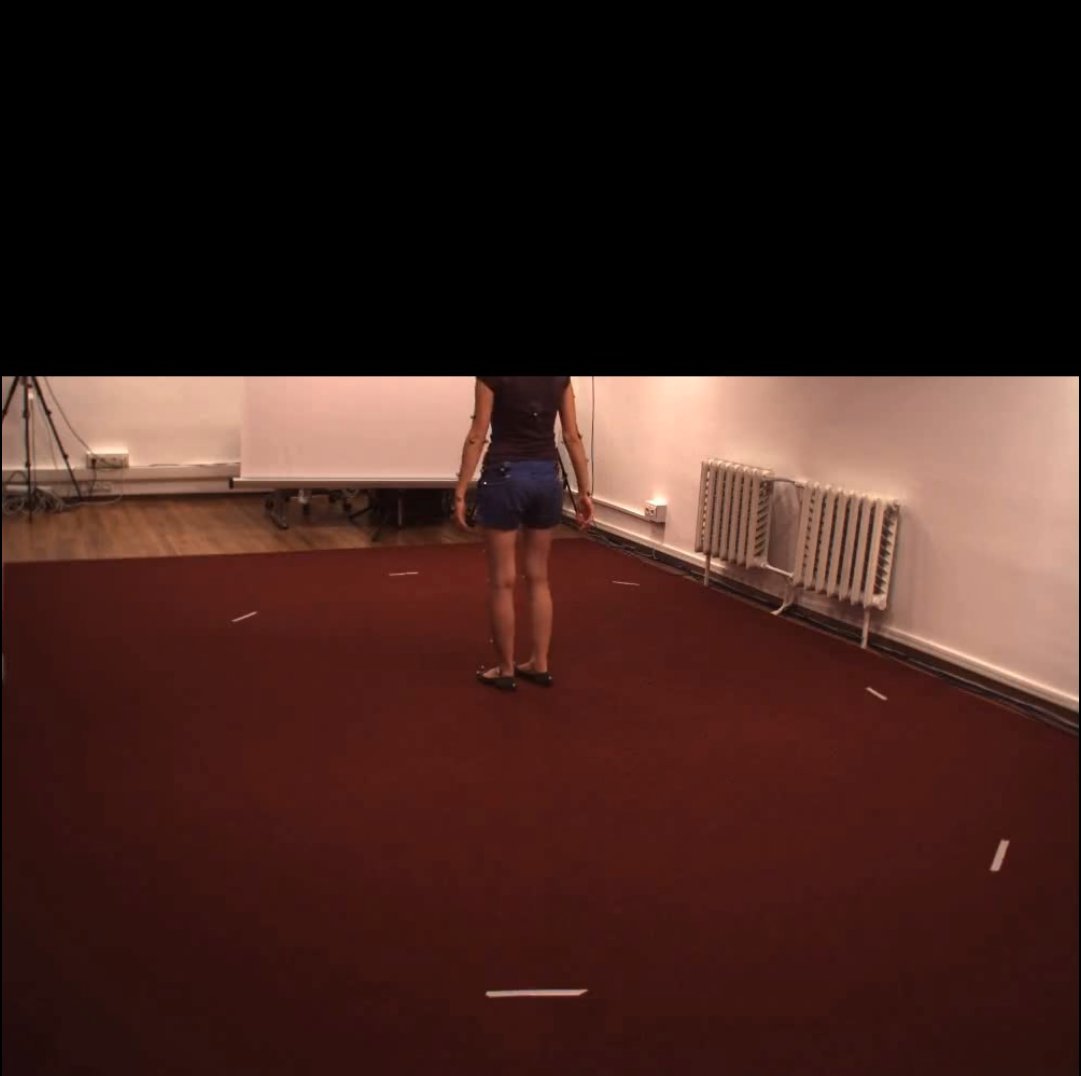
\includegraphics[width=\textwidth]{assets/h35_S1_Directions 1.54138969.png}
    \caption{Actor in the center, occlusion 0.35.}
    \label{fig: actor center, occlusion ratio 35}
  \end{subfigure}
  \begin{subfigure}[t]{0.24\textwidth}
    \centering
    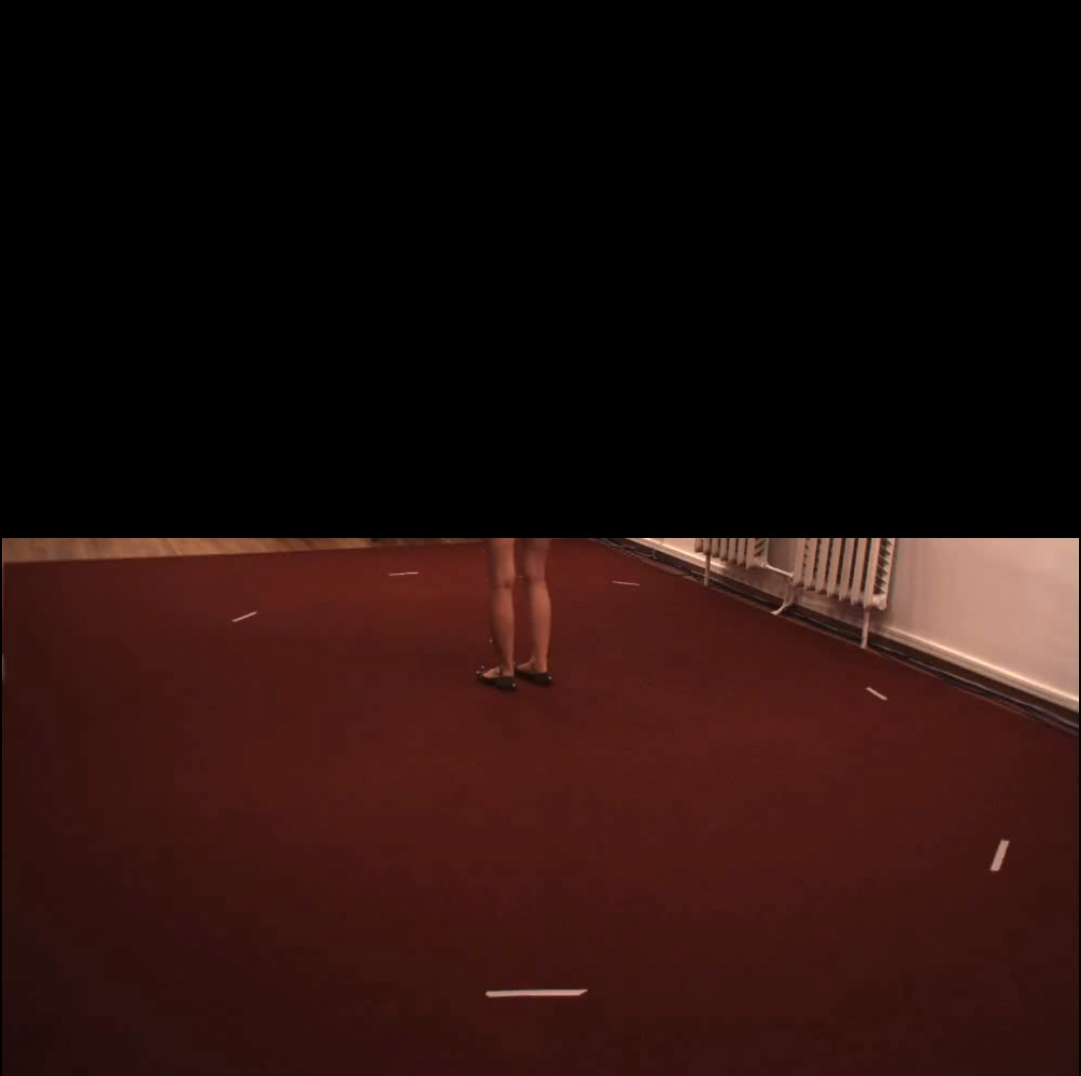
\includegraphics[width=\textwidth]{assets/h50_S1_Directions 1.54138969.png}
    \caption{Actor in the center, occlusion 0.50.}
    \label{fig: actor center, occlusion ratio 50}
  \end{subfigure}
  % \hfill
  \begin{subfigure}[t]{0.24\textwidth}
    \centering
    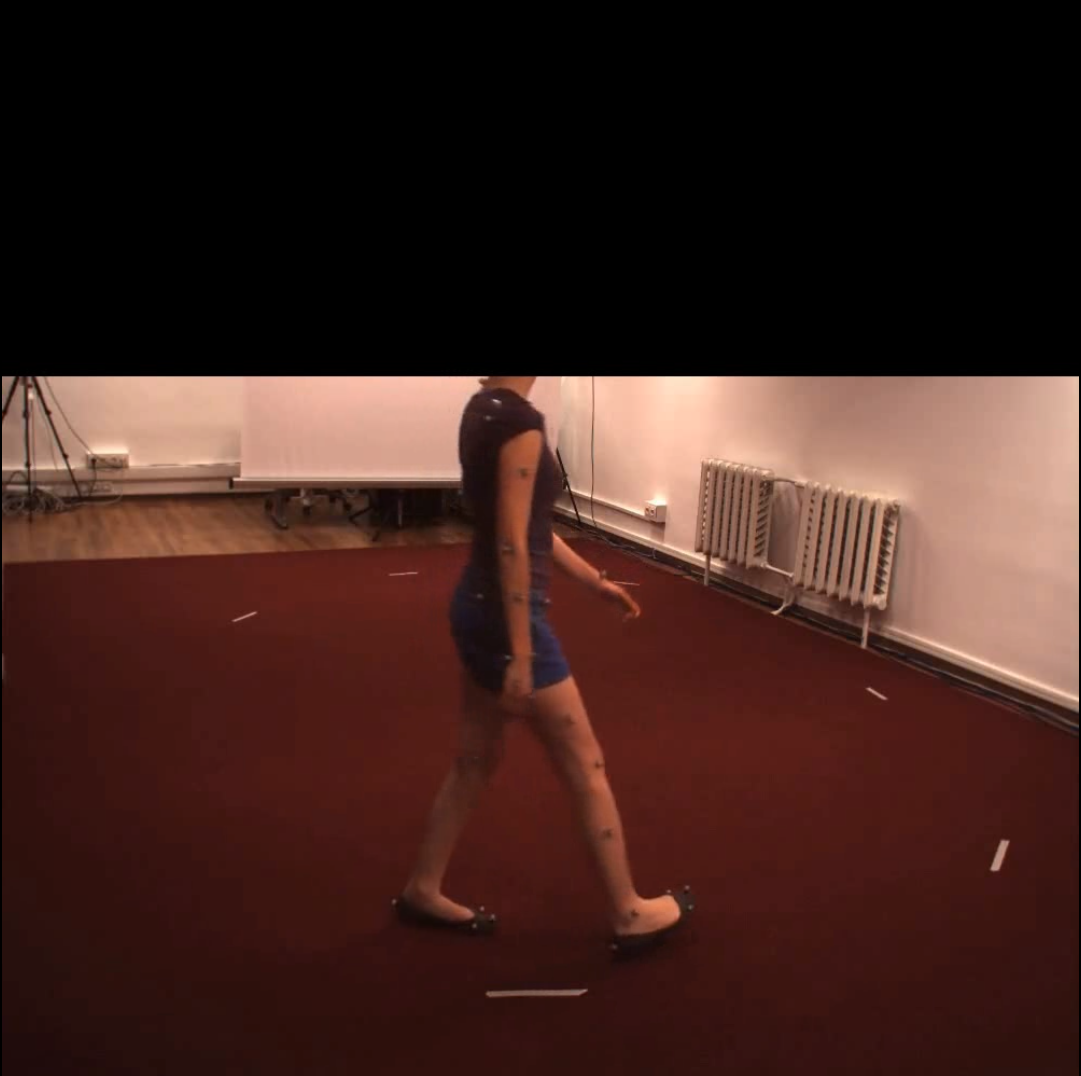
\includegraphics[width=\textwidth]{assets/h35_S1_Walking 1.54138969.png}
    \caption{Actor in the bottom, occlusion 0.35.}
    \label{fig: actor bottom, occlusion ratio 35}
  \end{subfigure}
  \begin{subfigure}[t]{0.24\textwidth}
    \centering
    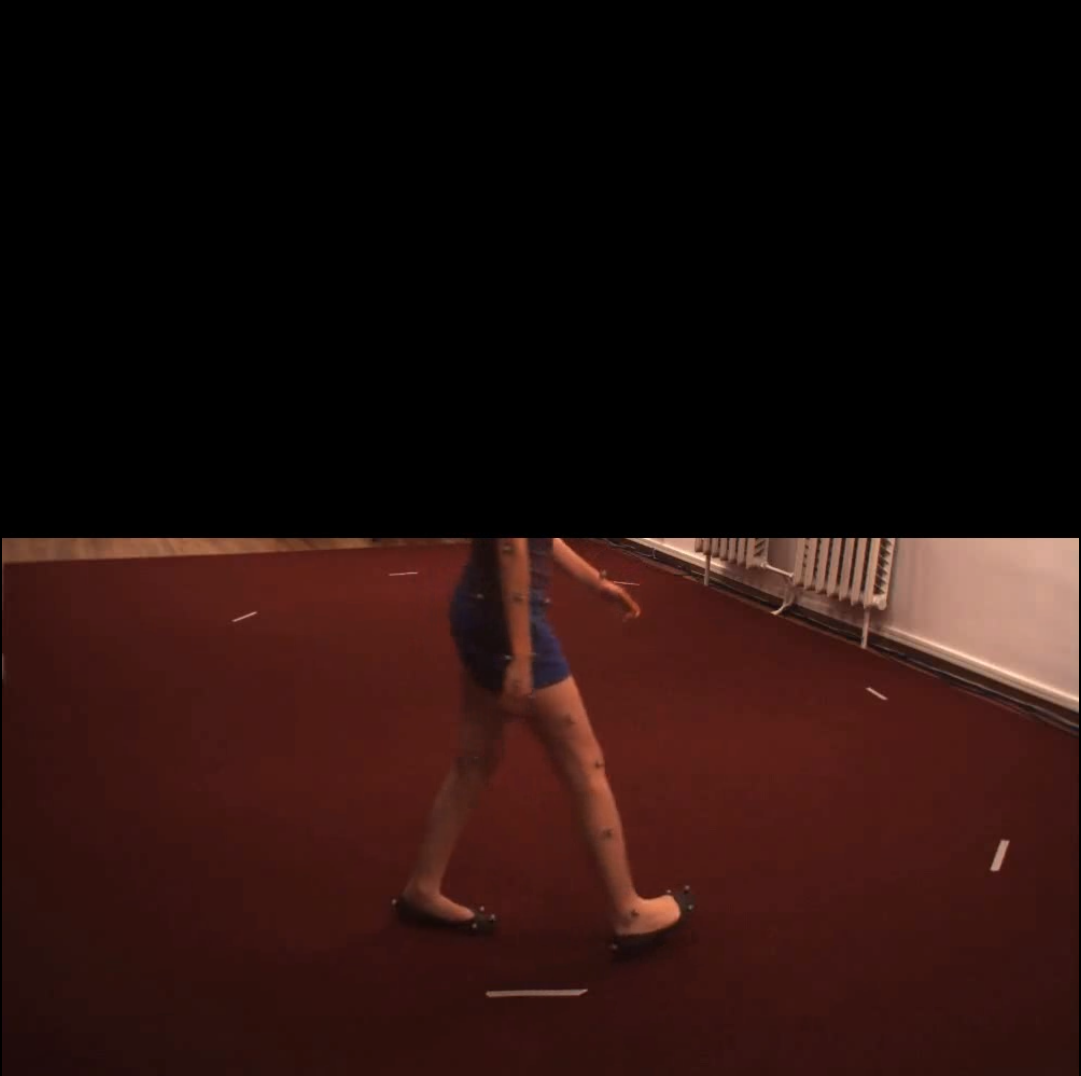
\includegraphics[width=\textwidth]{assets/h50_S1_Walking 1.54138969.png}
    \caption{Actor in the bottom, occlusion 0.50.}
    \label{fig: actor bottom, occlusion ratio 50}
  \end{subfigure}
  \caption{Comparison of occlusion ratios and actors positions. \ref{fig: actor center, occlusion ratio 35} vs \ref{fig: actor center, occlusion ratio 50} and \ref{fig: actor bottom, occlusion ratio 35} vs \ref{fig: actor bottom, occlusion ratio 50} compare occlusion ratios of 0.35 and 0.50 respectively. \ref{fig: actor center, occlusion ratio 35} vs \ref{fig: actor bottom, occlusion ratio 35} and \ref{fig: actor center, occlusion ratio 50} vs \ref{fig: actor bottom, occlusion ratio 50} compare actors positions in the center and at the bottom of the image respectively.}
  \label{fig: occlusion ratios and actors positions}
\end{figure}





\section{Datasets and Metrics}
Now that we introduced the approaches that can be used to identify people in images, we need two things: data and ways to evaluate these methods. Our first focus will be to present datasets, what they offer, why they could be interesting and their pitfalls. Then we will dive into the various metrics that exist in the 3D case, which also come with their share of strengths and weaknesses.

\subsection{Datasets}
One of the challenges when working on 3D images is to find appropriate datasets. Indeed, in comparison, the 2D setting has many datasets to offer, mainly because data collection and annotation is fairly easy. In the 3D world however, collecting data requires sensors to be placed on the protagonists' joints or heavy manual labeling. Indeed, annotating joints in the 3D space is also a harder task than in the 2D world. We will review a few datasets in depth, which may be of interest for our problem.
\paragraph{Human3.6M} \cite{Human3.6M} is a dataset containing 3.6 millions of 3D human poses along with their respective annotations from accurate sensors. These sensors were placed on 11 actors (6 men, 5 women) performing 17 tasks. The tasks being performed include smoking, taking photos and talking over the phone. There exists a conventional train-test-split called Protocol \#1 where subjects S1, S5, S6 and S7 are used for training and subjects S9 and S11 are used for testing. This dataset is commonly regarded as one of the most, if not the most, famous datasets for indoor 3D \ac{hpe}.

\paragraph{MPI-INF-3DHP} \cite{MPI-INF-3DHP} is a dataset of 1.3 million frames captured in a multi-camera, green screen setting. It encompasses 8 actors (4 men, 4 women) performing 8 types of action. Some of these actions are dynamic, such as exercising or doing sports, but some are not, like sitting on a chair or being on the ground. Thanks to the green screen setting, actors can easily be segmented, as well as modified (\textit{e.g.} augmented) in finalized clips. This dataset can also be easily downloaded from the internet.
\paragraph{MuPoTS-3D} \cite{MuPoTS-3D} is a multi-person 3D dataset of 8 people performing 20 real-world scenes, 5 of which are indoors and 15 of which are outdoors. It is a challenging dataset that contains numerous occlusions and lens flare in some outdoor images.

\subsection{Metrics}
We saw different approaches and datasets in this paper, but we need some common ground to evaluate them. Metrics in 3D \ac{hpe} are quite different from the usual accuracy, recall, f1-score that the data science community may be more used to. For this reason, we will detail them in this subsection.
\paragraph{\ac{mpjpe}} is the most commonly used metric to evaluate 3D \ac{hpe} algorithms. It is computed as the average 3D Euclidian distance between predicted joints and their respective ground truth. \\
Let $J_i$ and $J_i^*$ be the coordinates of the ground truth and prediction of the $i-th$ joint respectively. Let $N$ be the number of joints, then the \ac{mpjpe} is given by:
\begin{equation}
  MPJPE = \frac{1}{N} \sum_{i=1}^N \|J_i - J_i^*\|_2
\end{equation}

\paragraph{\ac{nmpjpe}} is similar to \ac{mpjpe}, but after normalizing the prediction coordinates with respect to the reference.

\paragraph{\ac{mpve}} computes the 3D Euclidian distance between the ground truth vertices and the predicted ones. \\
Let $V$ and $V_i^*$ be the ground truth and the predicted coordinates for the $i$-th vertex. Let $N$ be the number of vertices, then the \ac{mpve} is given by:
\begin{equation}
  MPVE = \frac{1}{N} \sum_{i=1}^N \|V_i - V_i^*\|_2
\end{equation}
According to some sources, \ac{mpjpe} depends on the predicted scale of human shape and skeleton, therefore it does not always accurately indicate an accurate pose \cite{survey}.

\paragraph{\ac{3dpck}} is a metric that considers that a joint is correcly identified if it lies closer that a given distance from ground truth, usually $150mm$. This metric turns the regression problem into a classification one, which may be more convenient for some applications.

\section{Evaluation and Comparison}
A summary of the best-performing techniques in each category can be found in Table \ref{table: presentation of results}. We note that having multiple views on the Human3.6M dataset almost halves the \ac{mpjpe} compared to single views. Comparing performances on different datasets is already tricky, but the fact that we do not have the same metrics for \ac{svsp} and \ac{svmp} simply makes the comparison impossible. One additional information on top of the table is that both best-performing skeleton techniques are lifting techniques rather than direct ones.
\begin{table}
  \centering
  \caption{Presentation of different, top-performing 3D \ac{hpe} techniques.}
  \label{table: presentation of results}
  \begin{tabular}{|cccccc|}
    \hline
    Task & Type      & Method                                          & Dataset                & Metric             & Score \\ \hline
    SVSP & Skeleton  & \cite{multi hypothesis transformer}             & Human3.6M (protocol 1) & MPJPE $\downarrow$ & 43.0  \\
    SVSP & Skeleton  & \cite{hrnet}                                    & Human3.6M (protocol 1) & MPJPE $\downarrow$ & 42.6  \\
    SVSP & HMR       & \cite{mesh reconstruction with transformers}    & Human3.6M (protocol 1) & MPJPE $\downarrow$ & 54.0  \\
    SVSP & HMR       & \cite{mesh graphormer}                          & Human3.6M (protocol 1) & MPJPE $\downarrow$ & 51.2  \\ \hline
    SVMP & Top-down  & \cite{HMOR}                                     & MuPoTS-3D              & 3DPCK $\uparrow$   & 82.0  \\
    SVMP & Top-down  & \cite{graph and temporal convolutional network} & MuPoTS-3D              & 3DPCK $\uparrow$   & 87.5  \\
    SVMP & Bottom-up & \cite{PandaNet}                                 & MuPoTS-3D              & 3DPCK $\uparrow$   & 72.0  \\
    SVMP & Bottom-up & \cite{SMAP}                                     & MuPoTS-3D              & 3DPCK $\uparrow$   & 73.5  \\ \hline
    MV   & -         & \cite{Transfusion}                              & Human3.6M              & MPJPE $\downarrow$ & 25.8  \\
    MV   & -         & \cite{MetaFuse}                                 & Human3.6M              & MPJPE $\downarrow$ & 29.3  \\
    \hline
  \end{tabular}
\end{table}

\section{Results \& analysis}
In section \ref{sec: methodology}, we stated that we wanted to answer several questions about \ac{svsp} methods: are they able to predict the occluded keypoints? Are they able to predict visible keypoints on occluded videos? How well do they predict visible keypoints on occluded compared to non-occluded videos? We will now answer these questions. What we call ``the model'' in subsequent paragraphs consists of the bottom-up detector, coupled to the lifter model we detailed in section \ref{sec: methodology}.
\paragraph{Ability to predict the occluded keypoints.}
The model is not able to infer occluded keypoints from the position of the visible ones. When trying to predict the occluded keypoints, the model seems to only predict them in the visible part of the image. This is probably due to the fact that the model is trained on non-occluded videos, and therefore does not have enough data to learn how to predict occluded keypoints. This deficiency suffers drastically from the increase of the number of occluded keypoints. Indeed, when the occlusion ratio is increased (figure \ref{fig: predictions varying occlusion ratios}), or when the subject moves towards the upper part of the image, the occluded keypoints stay in the visible part of the image, thus creating non-sensical predictions, such as predicting that the hands are next to the feet (figure \ref{fig: spider}).
\begin{figure}[ht]
  \centering
  \begin{subfigure}[t]{0.49\textwidth}
    \centering
    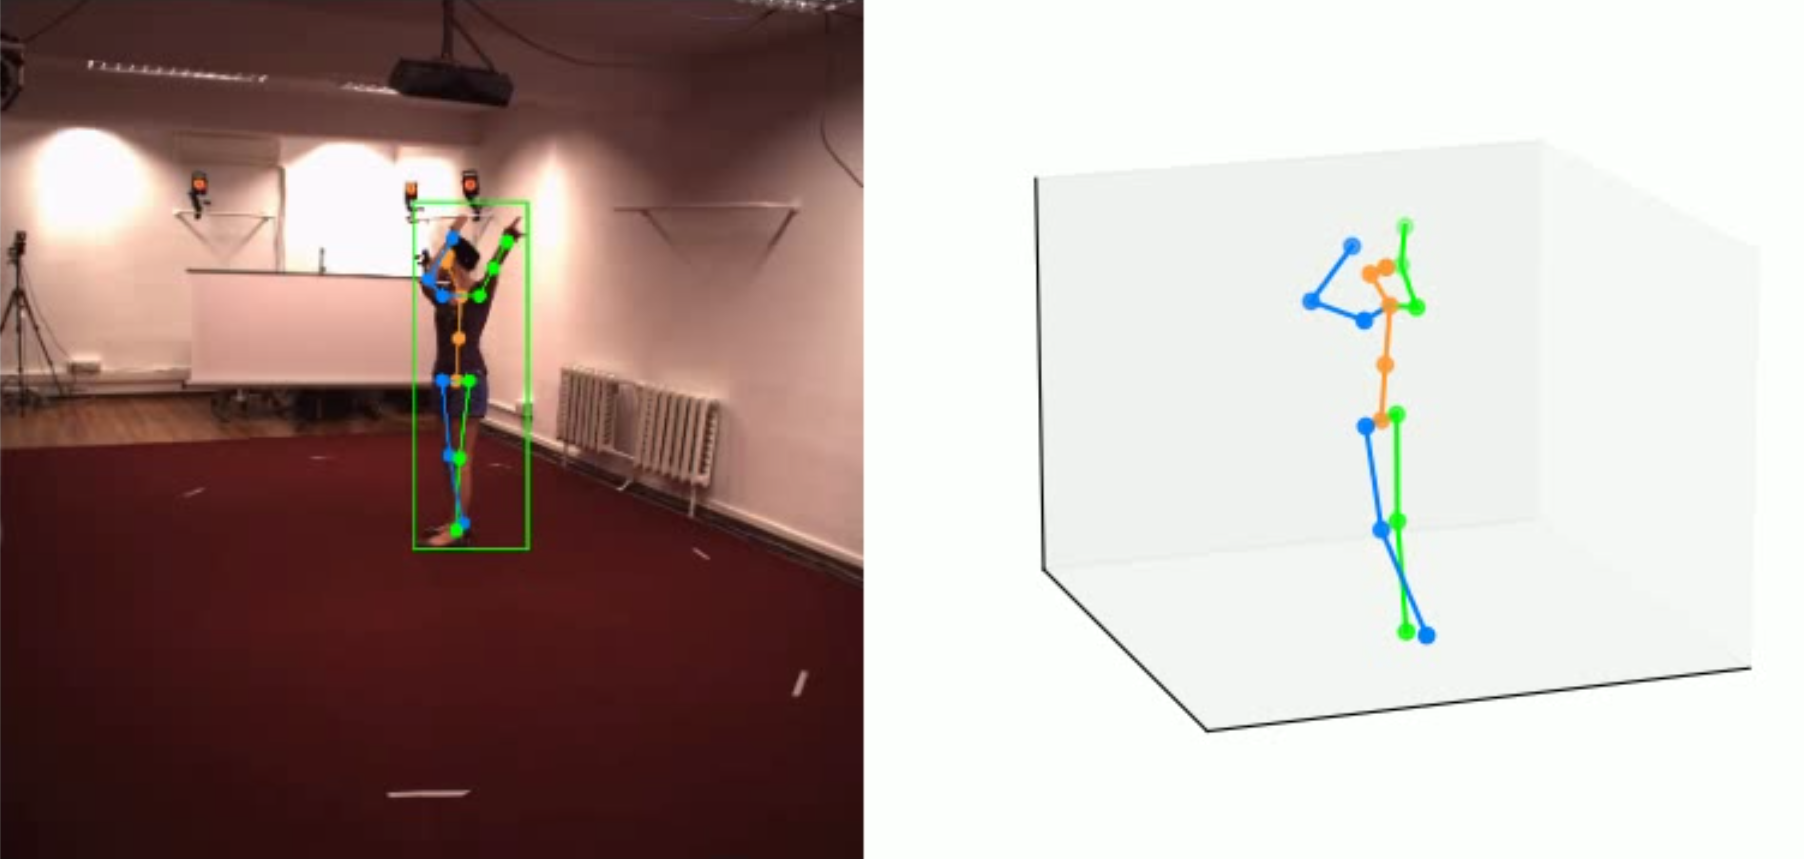
\includegraphics[width=\textwidth]{assets/pred_no_occlusion.png}
    \caption{Prediction without occlusion (occlusion ratio of 0).}
    \label{fig: no occlusion}
  \end{subfigure}
  \hfill
  \begin{subfigure}[t]{0.49\textwidth}
    \centering
    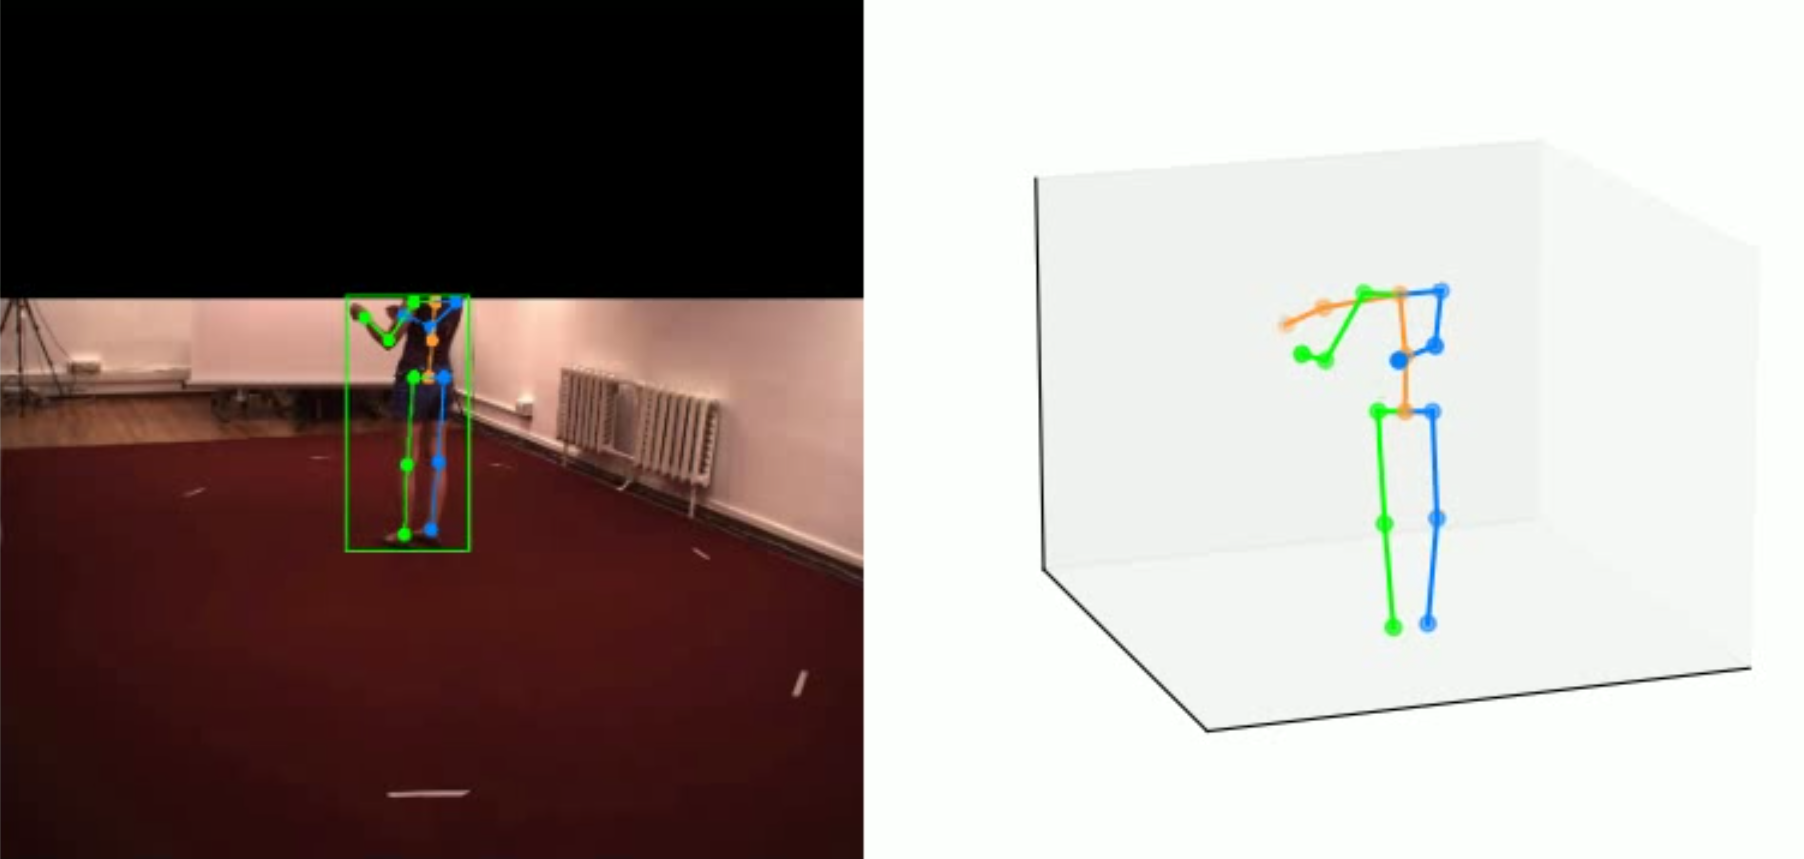
\includegraphics[width=\textwidth]{assets/pred_head_hidden.png}
    \caption{Prediction where the head is hidden (occlusion ratio of 0.35).}
    \label{fig: head hidden}
  \end{subfigure}
  \hfill
  \begin{subfigure}[t]{0.49\textwidth}
    \centering
    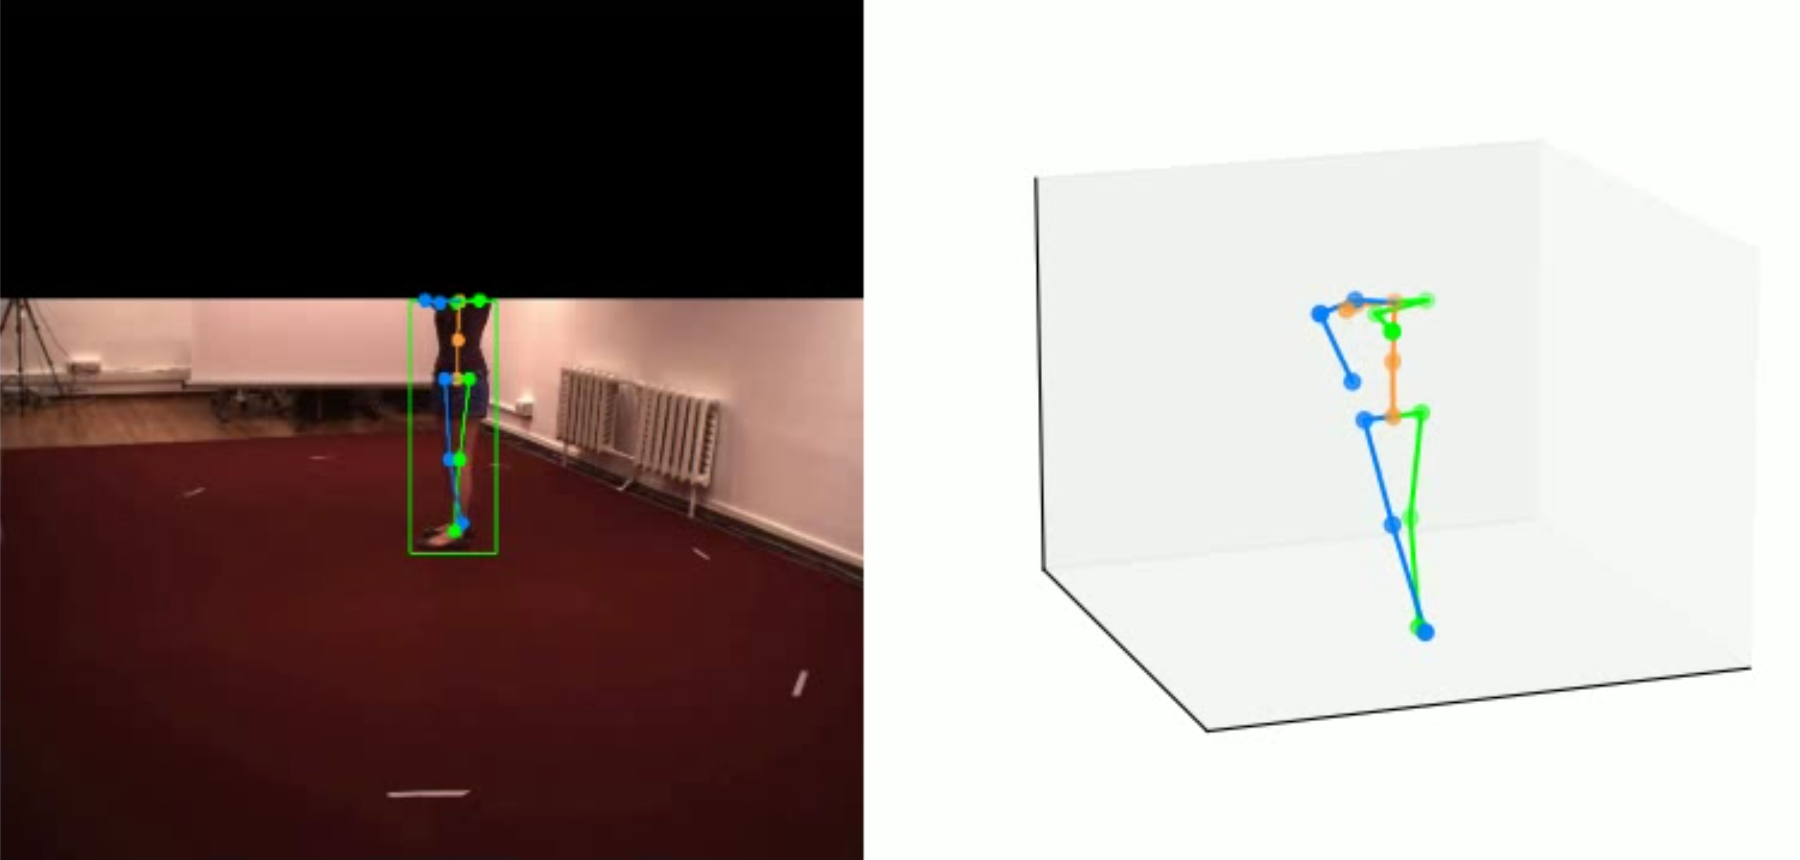
\includegraphics[width=\textwidth]{assets/pred_head_hidden_comp.png}
    \caption{Prediction where the head is hidden and the model fails to predict the legs (occlusion ratio of 0.35).}
    \label{fig: head hidden comp}
  \end{subfigure}
  \hfill
  \begin{subfigure}[t]{0.49\textwidth}
    \centering
    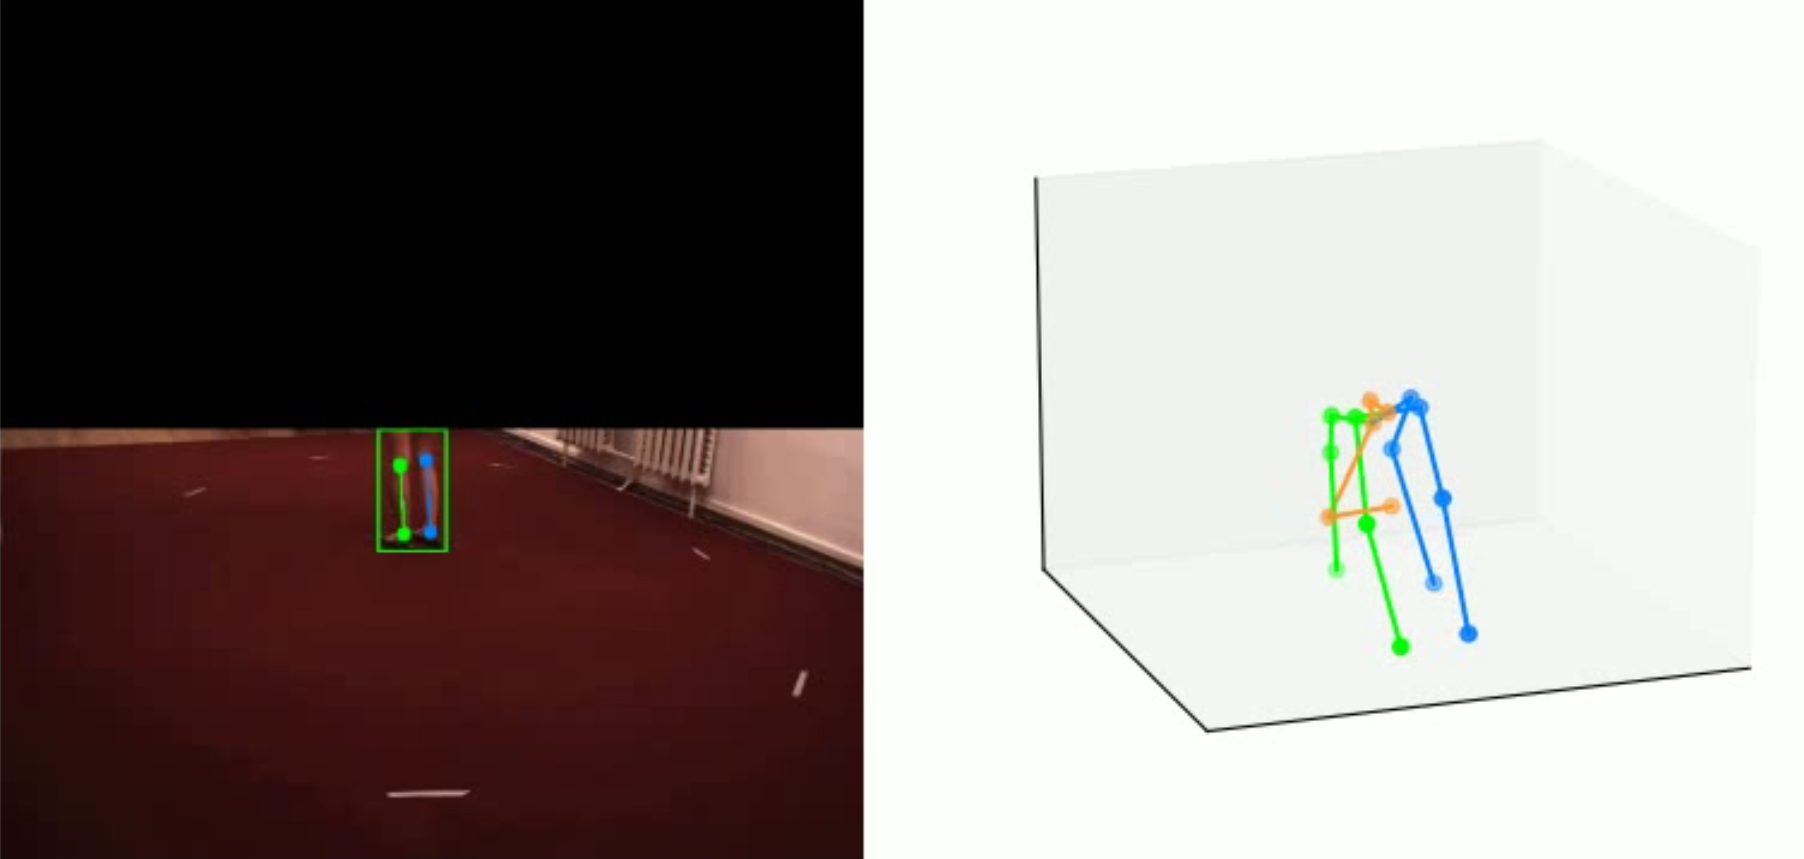
\includegraphics[width=\textwidth]{assets/pred_spider.png}
    \caption{Prediction where half of the body is hidden (occlusion ratio of 0.50).}
    \label{fig: spider}
  \end{subfigure}
  \caption{Predictions with varying occlusions ratios. The model is not able to predict the occluded keypoints. Instead, it tries to shift them in the visible part of the image.}
  \label{fig: predictions varying occlusion ratios}
\end{figure}

Table \ref{table: mpjpe varying occlusion ratios} shows the \ac{mpjpe} for the first 10 seconds of a given video (\textit{Directions 1.54138969.mp4}) for subject 1. We see that as the occlusion ratio increases, the \ac{mpjpe} also increases, which makes sense. However, we can say that the \ac{mpjpe} is not significantly higher for an occlusion ratio of 0.35 than for no occlusion. The largest increase occurs when we increase the occlusion ratio to 0.5, which we can easily understand since most of the actor's body is occluded and the model is not able to properly predict the keypoints. There are two things that qualify our results. First, this analysis is only done on a subclip of one video, so it is not a representative statistic. We did not compute more metrics by lack of time and lack of appropriate hardware. Second, the analysis was performed on all keypoints. Maybe a more interesting metric would have been to compute the \ac{mpjpe} only on visible keypoints. However, table \ref{table: mpjpe varying occlusion ratios} gives at least a hint at what the results may be on the whole test data.
\begin{table}
  \centering
  \begin{tabular}[t]{|c|c|}
    \hline
                    & MPJPE                 \\ \hline
    Occlusion ratio & Directions 1.54138969 \\ \hline
    0               & 322.39                \\
    0.35            & 326.17                \\
    0.50            & 441.72                \\ \hline
  \end{tabular}
  \caption{MPJPE of the model for varying occlusion ratios.}
  \label{table: mpjpe varying occlusion ratios}
\end{table}
\paragraph{Ability to predict visible keypoints on occluded videos.}
Although the visible keypoints may be cluttered and hard to distinguish in figure \ref{fig: spider}, the model still seems to be able to predict them somewhat coherently. This is further confirmed by figure \ref{fig: head hidden}, where the model is able to coherently predict the visible keypoints even though the head is hidden. Furthermore, we note that the model is unable to predict the legs in figure \ref{fig: head hidden comp} (left leg in green is wrongly predicted behind right leg in blue), however the model makes the same mistake in the non-occluded counterpart (figure \ref{fig: no occlusion}). This hints that wrong predictions on visible keypoints may not be due to occlusions, but rather to the model itself.
\paragraph{Prediction quality of visible keypoints on occluded compared to non-occluded videos.}
As mentioned previously, the prediction of visible keypoints in occluded scenes seems close enough to the prediction of visible keypoints in non-occluded scenes. However, it seems that the network is less confident about visible keypoints in occluded scenes, as can be noticed by their unstability. Indeed, the prediction of the keypoints seems to ``shake''. In other words, it appears that a high frequency noise is added to the joint position over time. This phenomenon is further amplified for occluded keypoints. \\

\section{Conclusion and Perspectives}
In this section, we make a recap about the results of this paper, and we discuss about a few ideas that may lead to future work.
\subsection{Conclusion}
Throughout this study of the State of the Art, we saw that 3D \ac{hpe} can be splitted into three tasks: \ac{svsp} , \ac{svmp} and \ac{mv}, which we detailed. The first one can consist of finding joints (skeleton) or superimposing an artificial 3D body model (\ac{hmr}). The second one can consist of either identifying each person in the image then finding their joints (top-down), or finding all joints plus a depth map before grouping these joints into the person they belong to (bottom-up). Finally, the last one avoids the strugles of other tasks, such as occlusions, thanks to its multiple views but it requires having multiple cameras and determining precisely where each of them lies with respect to the others. \\
We also saw that neither for datasets, nor for metrics is there one perfect, universal standard. For datasets, we have to choose between an ``easy'', maybe utopic, one and other ones with less data. For metrics, we may need to use several of them to properly evaluate the performances of any given model. \\
With respect to model predictions and occlusions, we answered three questions. The first one asked whether models are able to predict occluded keypoints. As we saw, they are not. Indeed, the occluded keypoints are predicted within the visible region of the image, although they are not visible. However, the results are not drastically worse as long as the occlusion is not pathological. \\
The second question asked whether models are able to predict visible keypoints on occluded videos. We saw that they are able to predict visible keypoints on occluded videos, but that they may be less confident about them. \\
The third question asked how well models predict visible keypoints on occluded compared to non-occluded videos. We saw that the prediction of visible keypoints in occluded scenes seems close enough to the prediction of visible keypoints in non-occluded scenes. Furthermore, we showcased an example where the model was unable to correctly predict the visible keypoints in the occluded setting, but it was also unable to correctly predict them in the non-occluded setting. However, we noted that the uncertainty of the network can be noticed through the high-frequency noise that is added to the joint position over time.


\subsection{Perspectives}
Building on that last challenge regarding the high-frequency noise, we could try to use the variance of a joint position over time as a metric to predict whether a keypoint is occluded or not. More variance in the joint position with respect to time could mean that the keypoint is occluded. This is not particularly interesting on the Human3.6M dataset because we add the synthetic occlusion ourselves, so we know which keypoints are occluded. However, it could be interesting for other datasets where is occlusion is more natural and unlabeled. For instance, in movie datasets where characters move in front of others and we want to predict the position of a character in the background. \\
Another simpler perspective would be to evaluate our model on visible keypoints only and on more videos. \\
Finally, a last perspective to improve the robustness of our model with respect to occlusions would simply be to train it on occluded videos. This may allow the model to learn how to predict occluded keypoints, as well as better predicting visible keypoints in occluded scenes.

\bibliographystyle{splncs04}
\begin{thebibliography}{8}
  \bibitem{survey} Zheng C, Wu W, Chen C, Yang T, Zhu S, Shen J, Kehtarnavaz N, Shah M (2022) Deep learning-based human pose estimation: A survey. In: \href{https://arxiv.org/abs/2012.13392}{arXiv.org. (link)}.
  \bibitem{multi hypothesis transformer} Li W, Liu H, Tang H, Wang P, Van Gool L. Mhformer: Multi-hypothesis transformer for 3d human pose estimation. InProceedings of the IEEE/CVF Conference on Computer Vision and Pattern Recognition 2022 (pp. 13147-13156).
  \bibitem{hrnet} Wang J, Yan S, Xiong Y, Lin D. Motion guided 3d pose estimation from videos. InEuropean Conference on Computer Vision 2020 Aug 23 (pp. 764-780). Springer, Cham. % 247
  \bibitem{R-CNN} He K, Zhang X, Ren S, Sun J. Deep residual learning for image recognition. InProceedings of the IEEE conference on computer vision and pattern recognition 2016 (pp. 770-778).
  \bibitem{Cascade R-CNN} Cai Z, Vasconcelos N. Cascade R-CNN: high quality object detection and instance segmentation. IEEE transactions on pattern analysis and machine intelligence. 2019 Nov 28;43(5):1483-98.
  \bibitem{FCOS} Tian Z, Shen C, Chen H, He T. Fcos: Fully convolutional one-stage object detection. InProceedings of the IEEE/CVF international conference on computer vision 2019 (pp. 9627-9636).
  \bibitem{CenterNet} Duan K, Bai S, Xie L, Qi H, Huang Q, Tian Q. Centernet: Keypoint triplets for object detection. InProceedings of the IEEE/CVF international conference on computer vision 2019 (pp. 6569-6578).
  \bibitem{Hybrid Task Cascade} Chen K, Pang J, Wang J, Xiong Y, Li X, Sun S, Feng W, Liu Z, Shi J, Ouyang W, Loy CC. Hybrid task cascade for instance segmentation. InProceedings of the IEEE/CVF Conference on Computer Vision and Pattern Recognition 2019 (pp. 4974-4983).
  \bibitem{Multi-view Pose transformer} Zhang J, Cai Y, Yan S, Feng J. Direct multi-view multi-person 3d pose estimation. Advances in Neural Information Processing Systems. 2021 Dec 6;34:13153-64.
  \bibitem{mesh reconstruction with transformers} Kevin Lin, Lijuan Wang, and Zicheng Liu. 2021. End-to-end human pose and mesh reconstruction with transformers. In CVPR. 1954–1963.
  \bibitem{mesh graphormer} Lin K, Wang L, Liu Z. End-to-end human pose and mesh reconstruction with transformers. InProceedings of the IEEE/CVF Conference on Computer Vision and Pattern Recognition 2021 (pp. 1954-1963).
  \bibitem{HMOR} Li J, Wang C, Liu W, Qian C, Lu CH. Hierarchical multi-person ordinal relations for monocular multi-person 3d pose estimation. arXiv 2020. arXiv preprint arXiv:2008.00206.
  \bibitem{graph and temporal convolutional network} Cheng Y, Wang B, Yang B, Tan RT. Graph and temporal convolutional networks for 3d multi-person pose estimation in monocular videos. InProceedings of the AAAI Conference on Artificial Intelligence 2021 May 18 (Vol. 35, No. 2, pp. 1157-1165).
  \bibitem{limb score} Zanfir A, Marinoiu E, Sminchisescu C. Monocular 3d pose and shape estimation of multiple people in natural scenes-the importance of multiple scene constraints. InProceedings of the IEEE Conference on Computer Vision and Pattern Recognition 2018 (pp. 2148-2157).
  \bibitem{bottom up 3D distance} Fabbri M, Lanzi F, Calderara S, Alletto S, Cucchiara R. Compressed volumetric heatmaps for multi-person 3d pose estimation. InProceedings of the IEEE/CVF Conference on Computer Vision and Pattern Recognition 2020 (pp. 7204-7213).
  \bibitem{PandaNet} Benzine A, Chabot F, Luvison B, Pham QC, Achard C. Pandanet: Anchor-based single-shot multi-person 3d pose estimation. InProceedings of the IEEE/CVF Conference on Computer Vision and Pattern Recognition 2020 (pp. 6856-6865).
  \bibitem{SMAP} Zhen J, Fang Q, Sun J, Liu W, Jiang W, Bao H, Zhou X. Smap: Single-shot multi-person absolute 3d pose estimation. InEuropean Conference on Computer Vision 2020 Aug 23 (pp. 550-566). Springer, Cham.
  \bibitem{Transfusion} Ma H, Chen L, Kong D, Wang Z, Liu X, Tang H, Yan X, Xie Y, Lin SY, Xie X. Transfusion: Cross-view fusion with transformer for 3d human pose estimation. arXiv preprint arXiv:2110.09554. 2021 Oct 18.
  \bibitem{MetaFuse} Xie R, Wang C, Wang Y. Metafuse: A pre-trained fusion model for human pose estimation. InProceedings of the IEEE/CVF Conference on Computer Vision and Pattern Recognition 2020 (pp. 13686-13695).
  \bibitem{Human3.6M} Ionescu C, Papava D, Olaru V, Sminchisescu C. Human3. 6m: Large scale datasets and predictive methods for 3d human sensing in natural environments. IEEE transactions on pattern analysis and machine intelligence. 2013 Dec 12;36(7):1325-39.
  \bibitem{MPI-INF-3DHP} Mehta D, Rhodin H, Casas D, Fua P, Sotnychenko O, Xu W, Theobalt C. Monocular 3d human pose estimation in the wild using improved cnn supervision. In2017 international conference on 3D vision (3DV) 2017 Oct 10 (pp. 506-516). IEEE.
  \bibitem{MuPoTS-3D} Mehta D, Sotnychenko O, Mueller F, Xu W, Sridhar S, Pons-Moll G, Theobalt C. Single-shot multi-person 3d pose estimation from monocular rgb. In2018 International Conference on 3D Vision (3DV) 2018 Sep 5 (pp. 120-130). IEEE.
  \bibitem{mmpose} MMPose Contributors. OpenMMLab Pose Estimation Toolbox and Benchmark, 2020. Available at: \url{https://github.com/open-mmlab/mmpose}.
  \bibitem{faster RCNN} Girshick, R., 2015. Fast r-cnn. In Proceedings of the IEEE international conference on computer vision (pp. 1440-1448).
  \bibitem{resnet} He, K., Zhang, X., Ren, S. and Sun, J., 2016. Deep residual learning for image recognition. In Proceedings of the IEEE conference on computer vision and pattern recognition (pp. 770-778).



\end{thebibliography}
\end{document}
